\chapter{Исследовательская часть}

В данном разделе будут приведены примеры работы программы, и будет проведен сравнительный анализ реализованных алгоритмов сортировки по затраченному процессорному времени.

\section{Технические характеристики}

Технические характеристики устройства, на котором выполнялось исследование, приведены ниже:

\begin{itemize}
	\item операционная система Manjaro Linux \cite{manjaro};
	\item память 7,6 ГБ;
	\item процессор 8 × Intel® Core™ i5-10210U CPU @ 1.60 ГГц \cite{intel}.
\end{itemize}

\clearpage

\section{Демонстрация работы программы}

На рисунке \ref{img:example} приведен пример работы программы. На этом рисунке пользователь выбирает из меню пункт 2 --- сортировку подсчетом, вводит исходный массив и получает на выходе отсортированный массив.

\begin{figure}[H]
	\begin{center}
		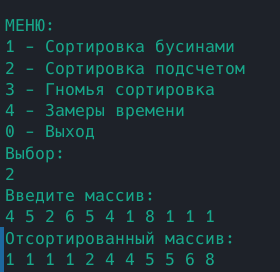
\includegraphics[scale=1]{img/example.png}
	\end{center}
	\captionsetup{justification=centering}
	\caption{Пример работы программы}
	\label{img:example}
\end{figure}

\section{Временные характеристики}

Функция process\_time\_ns из библиотеки time языка программирования Python возвращает  процессорное время в наносекундах.

Замеры проводились для массивов длиной от 100 до 1000.

На рисунке \ref{img:time_best} приведены результаты замеров времени алгоритмов сортировки для лучшего случая.

\begin{figure}[H]
	\begin{center}
		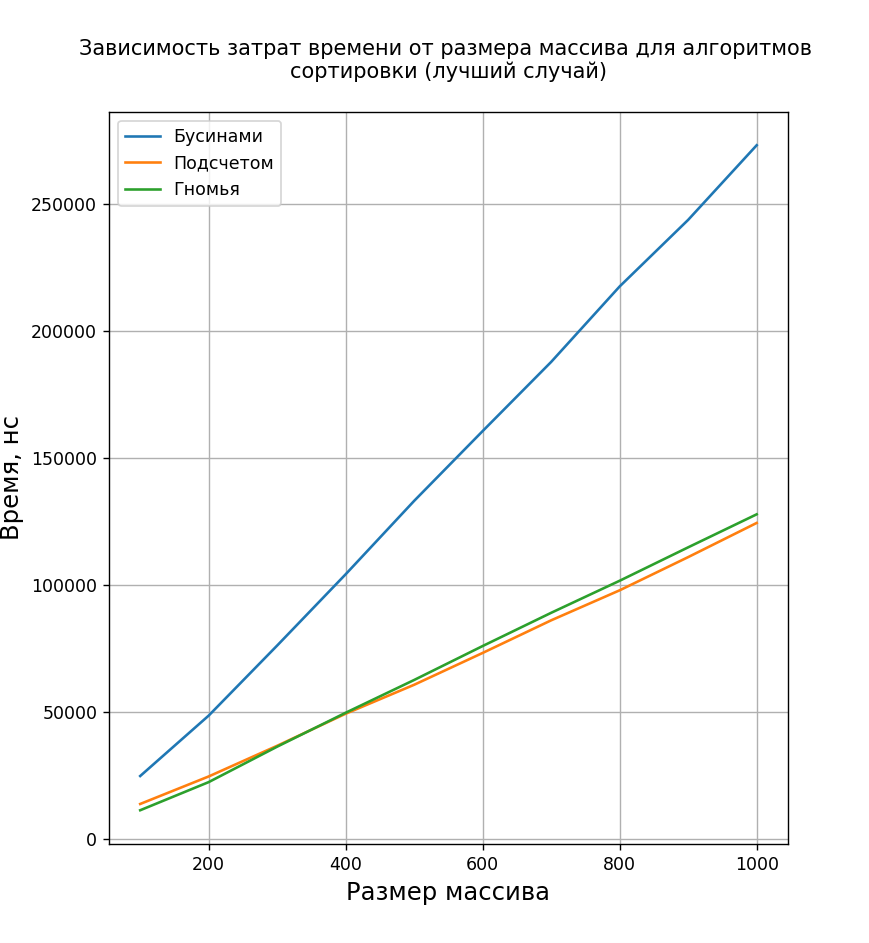
\includegraphics[scale=0.67]{img/time_best.png}
	\end{center}
	\captionsetup{justification=centering}
	\caption{Сравнение по времени алгоритмов сортировки (лучший случай)}
	\label{img:time_best}
\end{figure}

На рисунке \ref{img:time_worst} приведены результаты замеров времени алгоритмов сортировки для худшего случая.

\begin{figure}[H]
	\begin{center}
		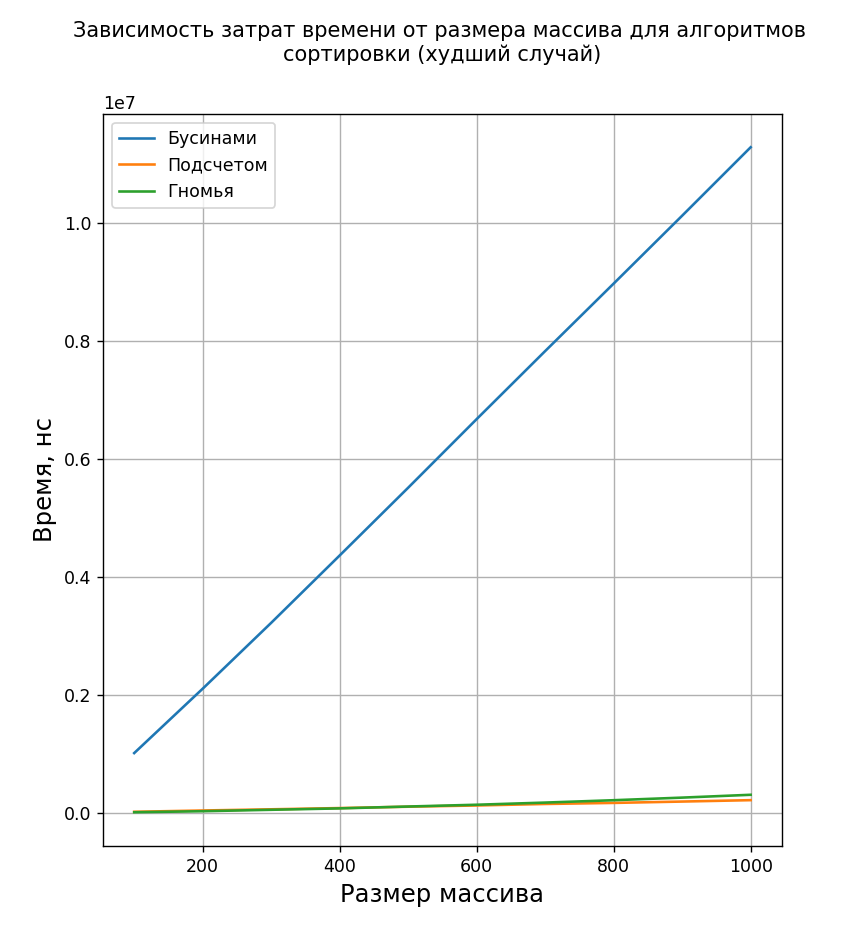
\includegraphics[scale=0.67]{img/time_worst.png}
	\end{center}
	\captionsetup{justification=centering}
	\caption{Сравнение по времени алгоритмов сортировки (худший случай)}
	\label{img:time_worst}
\end{figure}

На рисунке \ref{img:time_rand} приведены результаты замеров времени алгоритмов сортировки для произвольного случая.

\begin{figure}[H]
	\begin{center}
		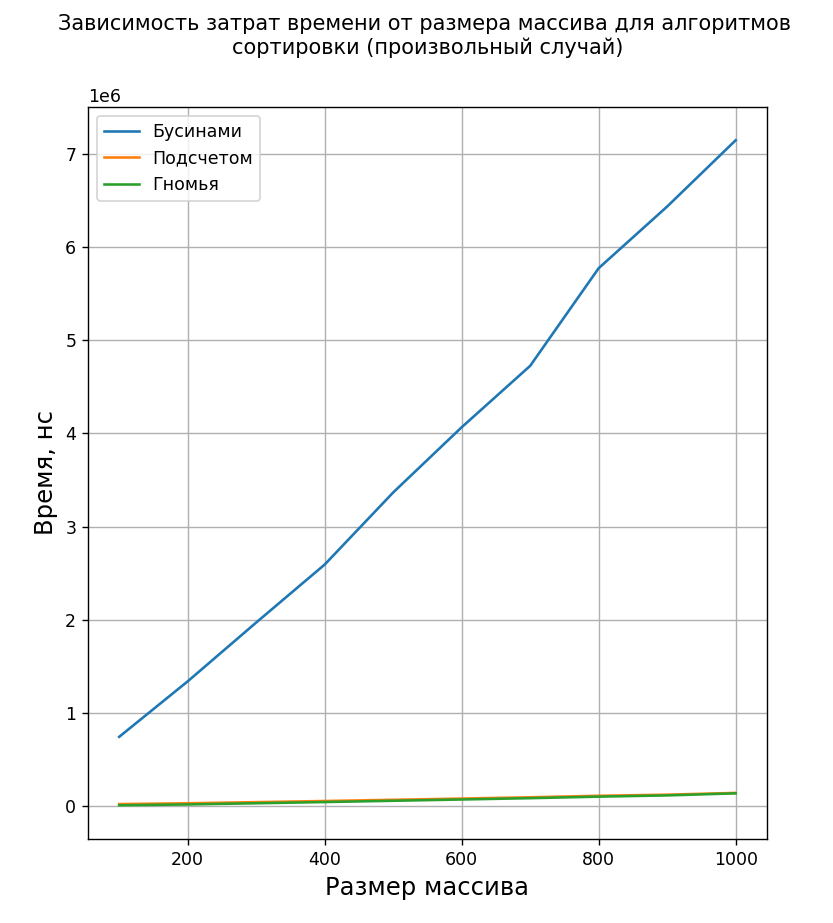
\includegraphics[scale=0.67]{img/time_rand.png}
	\end{center}
	\captionsetup{justification=centering}
	\caption{Сравнение по времени алгоритмов сортировки (произвольный случай)}
	\label{img:time_rand}
\end{figure}

\section{Вывод}
Приведенные характеристики времени показывают, что наименее эффективным по времени алгоритмом является сортировка бусинами. При этом результаты замеров времени для сортировки подсчетом и гномьей сортировки практически одинаковые для массивов, заполненных случайными элементами. Но для лучшего и худшего случаев выигрывает по времени сортировка подсчетом.